\section{Preprocesamiento}

Antes de iniciar con el proceso de construcción de \textit{embeddings} y modelos de clasificación se realizó una estandarización o preprocesamiento a los datos de ambos \textit{datasets}. Este se puede encontrar en el cuaderno adjunto  \texttt{preprocessing.iynb}. Se empezó por importar los diálogos de ambas series, los cuales se encontraban en formatos distintos. \\

Por un lado, para el \textit{dataset} de Los Simpsons, los datos ya se encontraban discriminados por personaje, por lo que el único trabajo que se hizo fue el de seleccionar los dialogos de los 4 personajes principales (Homero, Marge, Bart y Lisa Simpson). Por otro lado, para el \textit{dataset} de Friends, se tenían el script crudo de cada uno de los episodios. De esta manera se leyeron todos los archivos verificando su contenido en cada línea. En caso de encontrar alguno de los personajes principales (Rachel, Ross, Chandler, Monica, Joey o Phoebe) se agregaba el contenido seguido de los dos puntos \textit{(:)} y se le agregaba la etiqueta del personaje. \\

Así las cosas, se obtuvieron el siguiente número de sentencias (o frases) por cada uno de los personajes principales (véase cuadro \ref{tab:dist-datos}). En estas se observa que la distribución de las clases es similar para tres de los cuatro personajes de los Simpsons. No obstante, Homero acapara poco más del 40\% de las sentencias, lo que sugiere un desbalance considerable en el caso de este \textit{dataset}. Por el lado de la serie de Friends, se observa una distribución mucho más balanceada de las clases, con una diferencia menor al $4\%$ entre la clase con más datos y la de menos datos. \\

\begin{table}[H]
\caption{Distribución de las clases (número de sentencias para cada personaje) en cada uno de los \textit{datasets}.}
\label{tab:dist-datos}
\centering
\begin{minipage}{0.45\textwidth}
\centering
\begin{tabular}{|l|l|}
\hline
\textbf{Character} & \textbf{N° Sentences} \\ \hline
Homer & 27850 \\ \hline
Marge & 13172 \\ \hline
Bart & 12995 \\ \hline
Lisa & 10756 \\ \hline
\end{tabular}
\caption*{a) Simpsons }

\end{minipage}\hfill
\begin{minipage}{0.45\textwidth}
\centering
\begin{tabular}{|l|l|}
\hline
\textbf{Character} & \textbf{N° Sentences} \\ \hline
Rachel & 8506 \\ \hline
Ross & 8262 \\ \hline
Chandler & 7686 \\ \hline
Moncia & 7620 \\ \hline
Joey & 7572 \\ \hline
Phoebe & 6831 \\ \hline
\end{tabular}
\caption*{b) Friends}

\end{minipage}

\end{table}

Ahora bien, a cada una de las sentencias se les aplico una estandarización la cual consistió en los siguientes procesos:

\begin{itemize}
    \item \textbf{lower case:} Las letras de todos los términos se transformaron a minúsculas.
    
    \item \textbf{colloquial term removal:} Se expandieron contracciones coloquiales (ejemplo: la expreisón \textit{don't} se reemplazo por \textit{do not}).
    
    \item \textbf{tokenización:} Se tokenizaron las palabras con el tokenizador \texttt{RegexpTokenizer} de \texttt{nltk}, el cual elimina todo signo de puntuación.
        
    \item \textbf{simple lematization:} Se redujo cada uno de los términos a su raíz con el lematizador \texttt{WordNetLematizer} de \texttt{nltk}.
    
\end{itemize}

Dado que para este trabajo las palabras se modelaran con \textit{embeddings} y no con un modelo de palabras de \textit{Bag of Words} (BOW) el preprocesamiento fue realmente simple y no se decidió remover stop words. Una vez realizada esta estandarización se obtuvo el tamaño de las frases (número de tokens en cada sentencia) para cada uno de los \textit{datasets}. Esto con el fin de tener una idea de cuantos términos (o \textit{tokens}) había en cada frase (véase figura \ref{fig:simpsons_hist} - \ref{fig:friends_hist}), algo de especial importancia al momento de realizar el \textit{padding} de las sentencias.  \\

\begin{figure}[H]
    \centering
    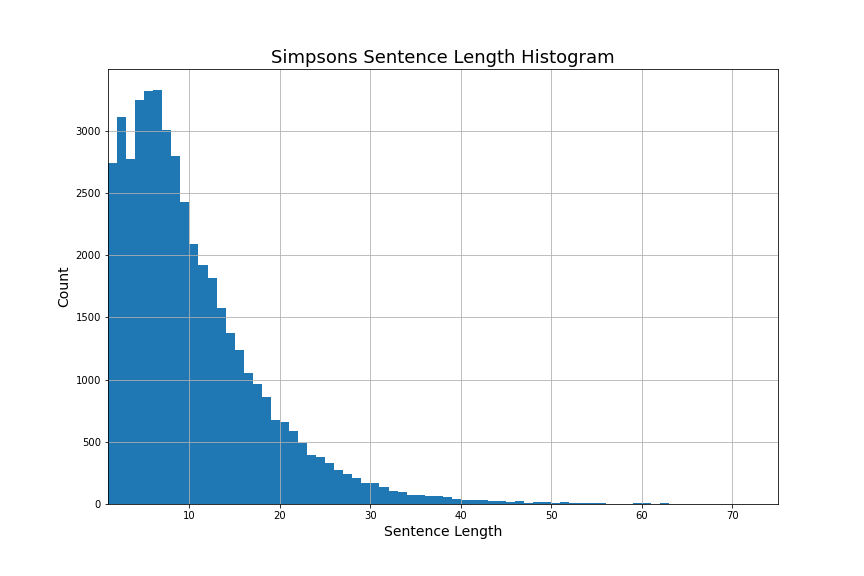
\includegraphics[width=0.95\textwidth]{results/preprocessing/simpsons_hist.png}
    \caption{Tamaño de las frases en los diálogos de los Simpsons (promedio = $9.93$, media = $8$).}
    \label{fig:simpsons_hist}
\end{figure}

Adicionalmente, en este punto también se separaron de una vez los \textit{datasets} en \textit{sets} de entrenamiento (\textit{train}), validación (\textit{val}) y prueba (\textit{test}), con una distribución de 70\%, 15\% y 15\% respectivamente. Esto con el fin de entrenar los modelos con un grupo de datos, definir su arquitectura y ajustar sus parámetros con otro grupo de datos y realizar la prueba definitiva de su desempeño con un último grupo de datos. 


\begin{figure}[H]
    \centering
    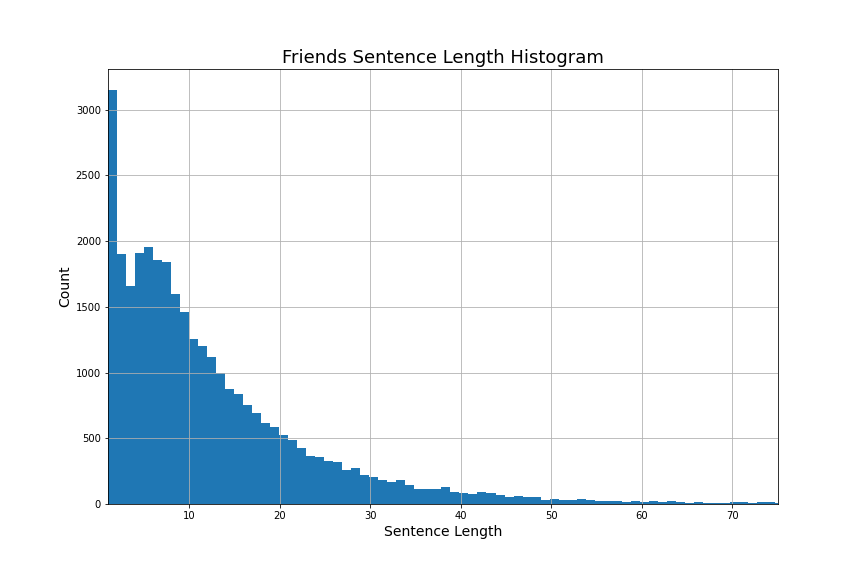
\includegraphics[width=0.95\textwidth]{results/preprocessing/friends_hist.png}
    \caption{Tamaño de las frases en los diálogos de la serie \textit{Friends} (promedio = $12.52$, media = $9$).}
    \label{fig:friends_hist}
\end{figure}

\newpage